% !TEX program = xelatex
\makeatletter\let\@expl@@@mark@update@singlecol@structures@@\relax\makeatother
\documentclass[a4paper,10pt]{article}

% -------------------- កញ្ចប់ពុម្ពអក្សរ និងភាសា --------------------
\usepackage{fontspec}
\usepackage{amsmath,amssymb}
\usepackage{unicode-math}
\usepackage{pifont}

% -------------------- ការកំណត់ទំព័រ (Page Setup — ម៉ូដ ls_plan.tex) --------------------
\usepackage[
  a4paper,
  left=0.95cm,
  right=0.95cm,
  top=0.85cm,
  bottom=0.92cm,
  footskip=0.52cm
]{geometry}

\usepackage{fancyhdr}
\usepackage{lastpage}
\usepackage{array}
\usepackage{longtable}
\usepackage{multirow}
\usepackage{colortbl}
\usepackage[table]{xcolor}
\usepackage{tikz}
\usetikzlibrary{calc,angles,quotes,arrows.meta,decorations.markings,patterns}
\usepackage{eso-pic}
\usepackage[most]{tcolorbox}

% -------------------- ពុម្ពអក្សរផ្លូវការ (Cross-Platform \NGSFindFonts) --------------------
\newcommand{\NGSFindFonts}{%
  \IfFileExists{C:/Windows/Fonts/cambria.ttc}{%
    \def\NGSSysPath{C:/Windows/Fonts/}%
    \def\NGSUserPath{C:/Users/KIT/AppData/Local/Microsoft/Windows/Fonts/}%
  }{%
    \IfFileExists{./fonts/KhmerOSsiemreap.ttf}{\def\NGSSysPath{./fonts/}\def\NGSUserPath{./fonts/}}{%
    \IfFileExists{../fonts/KhmerOSsiemreap.ttf}{\def\NGSSysPath{../fonts/}\def\NGSUserPath{../fonts/}}{%
    \IfFileExists{../../fonts/KhmerOSsiemreap.ttf}{\def\NGSSysPath{../../fonts/}\def\NGSUserPath{../../fonts/}}{%
    \IfFileExists{../../../fonts/KhmerOSsiemreap.ttf}{\def\NGSSysPath{../../../fonts/}\def\NGSUserPath{../../../fonts/}}{%
    \IfFileExists{../../../../fonts/KhmerOSsiemreap.ttf}{\def\NGSSysPath{../../../../fonts/}\def\NGSUserPath{../../../../fonts/}}{%
    \IfFileExists{../../../../../fonts/KhmerOSsiemreap.ttf}{\def\NGSSysPath{../../../../../fonts/}\def\NGSUserPath{../../../../../fonts/}}{%
    \IfFileExists{../../../../../../fonts/KhmerOSsiemreap.ttf}{\def\NGSSysPath{../../../../../../fonts/}\def\NGSUserPath{../../../../../../fonts/}}{%
      \def\NGSSysPath{../../../../../../../fonts/}\def\NGSUserPath{../../../../../../../fonts/}%
    }}}}}}}%
  }%
}
\NGSFindFonts

\setmathfont[Path={\NGSSysPath}, FontIndex=1, Scale=1.02]{cambria.ttc}
\defaultfontfeatures{Ligatures=TeX}

\setmainfont[
  Path={\NGSUserPath}, Extension=.ttf, Script=Khmer,
  BoldFont={KhmerOSsiemreap}, BoldFeatures={FakeBold=1.8},
  ItalicFont={KhmerOSsiemreap}, ItalicFeatures={FakeSlant=0.25},
  BoldItalicFont={KhmerOSsiemreap}, BoldItalicFeatures={FakeBold=1.8, FakeSlant=0.25}
]{KhmerOSsiemreap}

\newfontfamily\muol[Path={\NGSUserPath}, Extension=.ttf, Script=Khmer]{KhmerOSmuollight}
\newfontfamily\TimesEn[Path={\NGSSysPath}, Extension=.ttf, BoldFont={timesbd}, ItalicFont={timesi}, BoldItalicFont={timesbi}]{times}
\newfontfamily\NagaBold[Path={\NGSUserPath}, Extension=.ttf]{AKbalthom Naga Bold}
\newfontfamily\CalibriFont[Path={\NGSUserPath}, Extension=.ttf]{calibri}
\newfontfamily\Tacteing[Path={\NGSUserPath}]{TACTENG.TTF}
\newfontfamily\CourierBullet[Path={\NGSUserPath}, Extension=.ttf]{cour}
\newcommand{\wcirc}{{\CourierBullet\fontsize{9.5pt}{11pt}\selectfont o}}

\XeTeXlinebreaklocale "km"
\XeTeXlinebreakskip = 0pt plus 1pt minus 0.1pt

\definecolor{stepgray}{HTML}{D9D9D9}
\definecolor{headgray}{HTML}{F2F2F2}
\definecolor{boxgray}{HTML}{D9D9D9}
\definecolor{darkred}{HTML}{C00000}
\definecolor{red5e}{HTML}{FF0000}

\pagestyle{fancy}
\fancyhf{}
\renewcommand{\headrulewidth}{0pt}
\fancyfoot[R]{\CalibriFont\fontsize{10.5pt}{12pt}\selectfont\thepage}

\setlength{\parindent}{0pt}
\setlength{\parskip}{0pt}
\setlength{\tabcolsep}{3.8pt}
\setlength{\LTpre}{2pt}
\setlength{\LTpost}{2pt}

\newcolumntype{L}[1]{>{\raggedright\arraybackslash}p{#1}}
\newcolumntype{C}[1]{>{\centering\arraybackslash}p{#1}}

\newcommand{\en}[1]{{\TimesEn #1}}
\newcommand{\enbf}[1]{{\TimesEn\textbf{#1}}}
\newcommand{\unit}[1]{\,\text{\en{#1}}}
\newcommand{\fiveE}[1]{{\NagaBold\fontsize{9.5pt}{13pt}\selectfont\textcolor{red5e}{#1}}}
\newcommand{\timenote}[1]{\textcolor{darkred}{\textit{#1}}}
\newcommand{\redsub}[1]{\textcolor{darkred}{#1}}
\newcommand{\graybox}[1]{\colorbox{boxgray}{\strut\hspace{2pt}#1\hspace{2pt}}}
\newcommand{\ditem}{\tikz[baseline=-0.5ex]\fill (0,0.42ex) -- (0.42ex,0) -- (0,-0.42ex) -- (-0.42ex,0) -- cycle;\hspace{0.3em}}
\newcommand{\cnum}[1]{{\fontsize{10pt}{11pt}\selectfont\ding{\numexpr181+#1\relax}}\hspace{0.2em}}
\newcommand{\cfig}[1]{\par\vspace{2pt}{\centering #1\par}\vspace{2pt}}
\newcommand{\stepheader}[1]{\multicolumn{3}{|c|}{\cellcolor{stepgray}\muol #1} \\* \noalign{\hrule height 0.4pt}}
\newcommand{\khmflourish}{{\Tacteing\fontsize{36pt}{14pt}\selectfont\raisebox{-5pt}{3}}}

% ============================================================================
% បណ្ណាល័យរូបភាព TikZ ស-ខ្មៅ (Monochrome Print-Safe, Exact 7.55cm Width, Zero Overlap)
% ============================================================================
% ១. ជំហានទី២ រំលឹកមេរៀនចាស់៖ ចែកអុឺគ្លីតគ្មានសំណល់ (r = 0) និងតម្លៃខ្ទង់លេខ
\newcommand{\figPrereqDIVTwoOne}{%
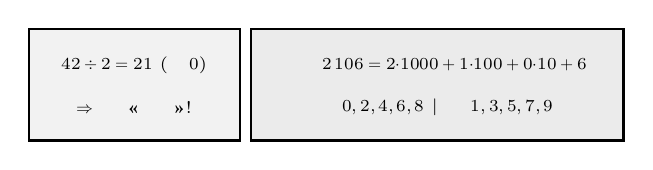
\begin{tikzpicture}[x=1cm, y=1cm, every node/.style={font=\fontsize{6.1pt}{8.1pt}\selectfont, text=black}]
  \draw[black, line width=0.85pt, fill=gray!10] (0,0) rectangle (2.68,1.42);
  \node at (1.34,0.96) {$42 \div 2 = 21$ (សល់ $0$)};
  \node at (1.34,0.42) {$\Rightarrow$ ហៅថា \textbf{«ចែកដាច់»}!};

  \draw[black, line width=0.85pt, fill=gray!16] (2.82,0) rectangle (7.55,1.42);
  \node at (5.185,0.96) {\textbf{ខ្ទង់៖} $2\,106 = 2{\cdot}1000 + 1{\cdot}100 + 0{\cdot}10 + 6$};
  \node at (5.185,0.42) {គូ៖ $0, 2, 4, 6, 8$ \textbar{} សេស៖ $1, 3, 5, 7, 9$};
\end{tikzpicture}}

% ២. E1 Engage: អន្ទាក់លេខខាងចុងរបស់ «ដារ៉ា» (23 ទល់នឹង 207)
\newcommand{\figEngageDIVTwoOne}{%
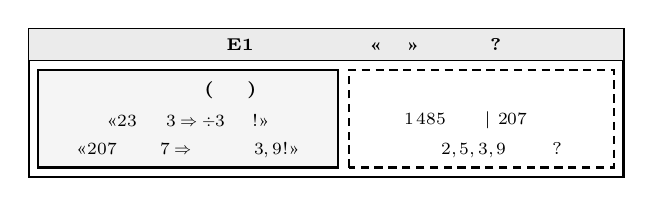
\begin{tikzpicture}[x=1cm, y=1cm, every node/.style={font=\fontsize{6.2pt}{8.2pt}\selectfont, text=black}]
  \draw[black, line width=0.9pt] (0,0) rectangle (7.55,1.88);
  \fill[gray!16] (0,1.48) rectangle (7.55,1.88);
  \draw[black, line width=0.6pt] (0,1.48) -- (7.55,1.48);
  \node at (3.775,1.68) {\textbf{បេសកកម្មឃ្លាំង \en{E1} ៖ តើការទស្សន៍ទាយរបស់ «ដារ៉ា» ត្រឹមត្រូវឬទេ?}};

  \draw[black, line width=0.75pt, fill=gray!8] (0.12,0.12) rectangle (3.92,1.36);
  \node at (2.02,1.10) {\textbf{ការអះអាងរបស់ដារ៉ា (អន្ទាក់)៖}};
  \node at (2.02,0.72) {«$23$ ចុង $3 \Rightarrow \div 3$ ដាច់!»};
  \node at (2.02,0.34) {«$207$ ចុងសេស $7 \Rightarrow$ មិនដាច់នឹង $3, 9$!»};

  \draw[black, line width=0.75pt, densely dashed, fill=white] (4.06,0.12) rectangle (7.43,1.36);
  \node at (5.745,1.10) {\textbf{សៀវភៅឃ្លាំងសាលា៖}};
  \node at (5.745,0.72) {$1\,485$ ក្បាល \textbar{} $207$ ក្បាល};
  \node at (5.745,0.34) {រៀបបាច់ $2, 5, 3, 9$ គ្មានសល់?};
\end{tikzpicture}}

% ៣. E2/E3: គំនូរតំណាង «កាក់សំណល់ពីបាច់ ១០ និង ១០០» (10=9+1, 100=99+1) ធៀបនឹងបាច់ 2 និង 5
\newcommand{\figBundleDIVTwoOne}{%
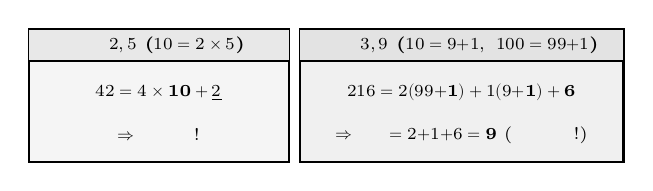
\begin{tikzpicture}[x=1cm, y=1cm, every node/.style={font=\fontsize{6.1pt}{8.0pt}\selectfont, text=black}]
  \draw[black, line width=0.85pt, fill=gray!8] (0,0) rectangle (3.30,1.68);
  \fill[gray!18] (0,1.28) rectangle (3.30,1.68);
  \draw[black, line width=0.55pt] (0,1.28) -- (3.30,1.28);
  \node at (1.65,1.48) {\textbf{ចែកនឹង $2, 5$ ($10 = 2\times 5$)}};
  \node at (1.65,0.88) {$42 = 4\times\mathbf{10} + \underline{2}$};
  \node at (1.65,0.34) {$\Rightarrow$ មើលតែ\textbf{រាយចុង}!};

  \draw[black, line width=0.85pt, fill=gray!12] (3.44,0) rectangle (7.55,1.68);
  \fill[gray!22] (3.44,1.28) rectangle (7.55,1.68);
  \draw[black, line width=0.55pt] (3.44,1.28) -- (7.55,1.28);
  \node at (5.495,1.48) {\textbf{ចែកនឹង $3, 9$ ($10=9{+}1,\ 100=99{+}1$)}};
  \node at (5.495,0.88) {$216 = 2(99{+}\mathbf{1}) + 1(9{+}\mathbf{1}) + \mathbf{6}$};
  \node at (5.495,0.34) {$\Rightarrow$ សំណល់ $= 2{+}1{+}6 = \mathbf{9}$ (បូកគ្រប់ខ្ទង់!)};
\end{tikzpicture}}

% ៤. E3 Venn: ទំនាក់ទំនងចែកដាច់នឹង 9 ទល់នឹង 3 និងប្រភេទទាំង ២
\newcommand{\figVennDIVTwoOne}{%
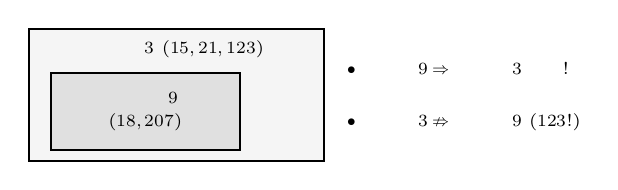
\begin{tikzpicture}[x=1cm, y=1cm, every node/.style={font=\fontsize{6.2pt}{8.1pt}\selectfont, text=black}]
  \draw[black, line width=0.85pt, fill=gray!8] (0,0) rectangle (3.75,1.68);
  \draw[black, line width=0.85pt, fill=gray!24] (0.28,0.14) rectangle (2.68,1.12);
  \node at (1.875,1.42) {\textbf{ចែកដាច់នឹង $3$} ($15, 21, 123$)};
  \node[align=center] at (1.48,0.63) {\textbf{ចែកដាច់នឹង $9$}\\($18, 207$)};

  \node[anchor=west, align=left] at (3.92,1.18) {$\bullet$ ចែកដាច់នឹង $9 \Rightarrow$ ចែកដាច់នឹង $3$ \textbf{ជានិច្ច}!};
  \node[anchor=west, align=left] at (3.92,0.50) {$\bullet$ ចែកដាច់នឹង $3 \not\Rightarrow$ ចែកដាច់នឹង $9$ ($123$!)};
\end{tikzpicture}}

% ៥. E5 Code Puzzle: ល្បែងបំបែកកូដសោសុវត្ថិភាព 526□
\newcommand{\figCodeDIVTwoOne}{%
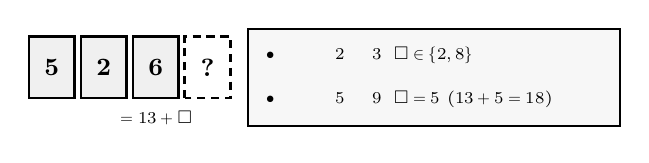
\begin{tikzpicture}[x=1cm, y=1cm, every node/.style={font=\fontsize{6.0pt}{8.0pt}\selectfont, text=black}]
  \foreach \x/\d in {0.04/5, 0.70/2, 1.36/6} {
    \draw[black, line width=0.85pt, fill=gray!12] (\x,0.42) rectangle (\x+0.58,1.20);
    \node[font=\small] at (\x+0.29,0.81) {\textbf{\d}};
  }
  \draw[black, line width=1.05pt, densely dashed, fill=white] (2.02,0.42) rectangle (2.60,1.20);
  \node[font=\small] at (2.31,0.81) {\textbf{?}};
  \node at (1.32,0.16) {ផលបូកខ្ទង់ $= 13 + \square$};

  \draw[black, line width=0.75pt, fill=gray!6] (2.82,0.06) rectangle (7.55,1.30);
  \node[anchor=west] at (2.94,0.96) {$\bullet$ ចែកដាច់នឹង $2$ និង $3$៖ $\square \in \{2, 8\}$};
  \node[anchor=west] at (2.94,0.40) {$\bullet$ ចែកដាច់នឹង $5$ និង $9$៖ $\square = 5$ ($13+5=18$)};
\end{tikzpicture}}

% ============================================================================
% ចាប់ផ្ដើមឯកសារ (Document Body)
% ============================================================================
\begin{document}
\fontsize{10pt}{15.2pt}\selectfont

% -------------------- ក្បាលកិច្ចតែងការ (Header) --------------------
\begin{center}
  {\muol\fontsize{11pt}{16pt}\selectfont ព្រះរាជាណាចក្រកម្ពុជា}\\[2pt]
  {\muol\fontsize{10pt}{15pt}\selectfont ជាតិ សាសនា ព្រះមហាក្សត្រ}\\[1pt]
  \khmflourish
\end{center}

\vspace{-28pt}
{\muol\fontsize{9.5pt}{12.5pt}\selectfont
មន្ទីរអប់រំ យុវជន និងកីឡា ខេត្តកំពង់ធំ\\
ការិយាល័យអប់រំ យុវជន និងកីឡា ស្រុកកំពង់ស្វាយ\\
អនុវិទ្យាល័យព្រះក្រសាំង}

\vspace{1pt}
\begin{center}
  {\muol\fontsize{10pt}{14pt}\selectfont កិច្ចតែងការបង្រៀន}
\end{center}
\vspace{0pt}

% -------------------- ព័ត៌មានទូទៅ (Metadata) --------------------
{\renewcommand{\arraystretch}{0.95}
\hspace*{4.05cm}%
\begin{tabular}{@{}l l l@{}}
  - \hspace{0.35cm} មុខវិជ្ជា & : & គណិតវិទ្យា ថ្នាក់ទី៧ \\
  - \hspace{0.35cm} ចំណងជើងមេរៀន & : & មេរៀនទី២ តួចែកនិងពហុគុណ \\
  - \hspace{0.35cm} ចំណងជើងរង & : & ១.១ ភាពចែកដាច់នឹង ២, ៥ និង ៣, ៩ (ទំ.១៥--១៦) \\
  - \hspace{0.35cm} រយៈពេល & : & ១ ម៉ោងសិក្សា (៥០ នាទី) \\
  - \hspace{0.35cm} បង្រៀនដោយ & : & ហុក ប៊ុនថែន \\
  - \hspace{0.35cm} កាលបរិច្ឆេទ & : & ថ្ងៃព្រហស្បតិ៍ ទី១២ ខែវិច្ឆិកា ឆ្នាំ២០២៦ \\
\end{tabular}

\vspace{1pt}

% -------------------- I. វត្ថុបំណង --------------------
\textbf{I.} {\muol វត្ថុបំណង}\\[1pt]
\hspace*{0.55cm}%
\begin{tabular}{@{}l l L{14.2cm}@{}}
  \wcirc \hspace{0.25cm} វិជ្ជាសម្បទា & : & សិស្សប្រាប់លក្ខណៈចែកដាច់នៃចំនួនគត់នឹង $2, 5, 3, 9$ និងពន្យល់មូលហេតុដែលលេខខ្ទង់រាយកំណត់ភាពចែកដាច់នឹង $2, 5$ រីឯផលបូកខ្ទង់លេខកំណត់ភាពចែកដាច់នឹង $3, 9$ បានត្រឹមត្រូវ ។ \\
  \wcirc \hspace{0.25cm} បំណិនសម្បទា & : & សិស្សប្រើតារាងពិសោធន៍ខ្ទង់ដប់--រាយ និងវិធានបូកខ្ទង់លើសន្លឹកកិច្ចការ ដើម្បីកំណត់ភាពចែកដាច់នៃចំនួនធំ ផលបូក និងបំពេញលេខក្នុងប្រអប់ឱ្យចែកដាច់នឹង $2, 5, 3, 9$ ដោយមិនធ្វើវិធីចែក ។ \\
  \wcirc \hspace{0.25cm} ចរិយាសម្បទា & : & សិស្សមានភាពប្រុងប្រយ័ត្នមិនច្រឡំមើលតែលេខខាងចុងសម្រាប់ក្បួន $3, 9$ មានទម្លាប់ផ្ទៀងផ្ទាត់ហេតុផលលេខវិទ្យា និងសហការរួមគិតប្រកបដោយសណ្ដាប់ធ្នាប់ ។ \\
\end{tabular}

\vspace{1pt}

% -------------------- II. សម្ភារៈឧបទេស --------------------
\textbf{II.} {\muol សម្ភារៈឧបទេស}\\[1pt]
\hspace*{0.55cm}$\bullet$ \hspace{0.35cm} សៀវភៅសិក្សាគោលថ្នាក់ទី៧ (ទំ.១៥--១៦) ក្ដារខៀន ដីស បន្ទាត់ និង\textbf{សន្លឹកកិច្ចការសិស្ស ស-ខ្មៅ (\en{Worksheet\_DIV21} ទំព័រ ១--២)} (គ្មានស្លាយ \en{LCD})

\vspace{1pt}

% -------------------- III. វិធីសាស្រ្តបង្រៀន --------------------
\textbf{III.} {\muol វិធីសាស្រ្តបង្រៀន}\\[1pt]
\hspace*{0.45cm}%
\begin{tabular}{@{}l l L{14.85cm}@{}}
  $\bullet$ \hspace{0.25cm} គោលវិធី & : & សិស្សមជ្ឈមណ្ឌល (ផ្អែកលើសន្លឹកកិច្ចការពិសោធន៍បាច់ដប់--រាយ និងល្បែងបំបែកកូដលេខ ស-ខ្មៅ គ្មាន \en{LCD}) \\
  $\bullet$ \hspace{0.25cm} យុទ្ធវិធីបង្រៀន & : & គំរូ 5Es រួមផ្សំការស្វែងរកគំរូលេខ (\en{Pattern Inquiry}) ការបកស្រាយកាក់សំណល់ និងសំណួរត្រិះរិះ \en{EIA} \\
\end{tabular}
}

\vspace{1pt}

% -------------------- IV. ដំណើរការបង្រៀន --------------------
\textbf{IV.} {\muol ដំណើរការបង្រៀន}

\vspace{1pt}

\renewcommand{\arraystretch}{1.12}
\begin{longtable}{|L{5.50cm}|L{7.90cm}|L{4.80cm}|}
\hline
\rowcolor{headgray}
\multicolumn{1}{|c|}{\muol សកម្មភាពគ្រូ} &
\multicolumn{1}{c|}{\muol ខ្លឹមសារមេរៀន} &
\multicolumn{1}{c|}{\muol សកម្មភាពសិស្ស} \\
\hline
\endfirsthead

\hline
\endhead

\hline
\endfoot

\hline
\endlastfoot

% ==================== ជំហានទី១ (2min) ====================
\stepheader{ជំហានទី១ \enbf{(}រដ្ឋបាលថ្នាក់\enbf{)}}
$\bullet$ ពិនិត្យអវត្តមាន សណ្ដាប់ធ្នាប់ អនាម័យ និងការត្រៀមសៀវភៅសិក្សាគោលថ្នាក់ទី៧
&
$\bullet$ រដ្ឋបាលថ្នាក់ និងការត្រៀមខ្លួនចូលរៀនមេរៀនទី២ (តួចែកនិងពហុគុណ)
&
$\circ$ ប្រធានថ្នាក់រាយការណ៍អវត្តមាន និងរៀបចំតុឱ្យមានរបៀប \\[2pt]

$\bullet$ ចែក \textbf{សន្លឹកកិច្ចការ ២.១} (ទំព័រ ១--២ ស-ខ្មៅ) ជូនសិស្សគ្រប់គ្នាផ្កាប់លើតុ
&
$\bullet$ សន្លឹកកិច្ចការសិស្សស្ដីពីភាពចែកដាច់នឹង $2, 5, 3, 9$ (គ្មានស្លាយ \en{LCD})
&
$\circ$ ទទួលសន្លឹកកិច្ចការផ្កាប់ទុកលើតុ \\[2pt]
\hline

% ==================== ជំហានទី២ (9min: <=3 + 3 + E1 3) ====================
\stepheader{ជំហានទី២ \enbf{(}ពិនិត្យចំណេះដឹងមុន \enbf{+} ទំនាក់ទំនងមេរៀនថ្មី\enbf{)}}
\ditem \textbf{ពិនិត្យកិច្ចការផ្ទះ ($\le 3\unit{min}$)} \timenote{ផ្ទៀងគន្លឹះលើក្ដារខៀន} \par
$\bullet$ ហៅសិស្ស ២ នាក់សរសេរចម្លើយសង្ខេបលេខ ៨ និង លេខ ៩ (មេរៀនទី១ ទំ.១៤)
&
{\centering\redsub{កំណែសង្ខេបមេរៀនទី១ (ទំ.១៤ លេខ ៨ និង លេខ ៩)}\par}
$\bullet$ \textbf{លេខ ៨៖} ក. $\graybox{$500$}$\; ខ. $\graybox{$134$}$\; គ. $\graybox{$37$}$\; ឃ.~\mbox{$3(5)^2=\graybox{$75$}$~\text{។}} \par
$\bullet$ \textbf{លេខ ៩៖} ក. $\graybox{$12$}$\; ខ. $\graybox{$14$}$\; គ. $\graybox{$140$}$\; ឃ.~\mbox{$\graybox{$\frac{127}{27}$}$~\text{។}}
&
$\circ$ ផ្ទៀងផ្ទាត់ចម្លើយលេខ ៨--៩ ក្នុងសៀវភៅកិច្ចការផ្ទះ \\[2pt]

\ditem \textbf{រំលឹកមេរៀនទាក់ទង (3min)} \timenote{សរុបកុំឱ្យលើស 3min} \par
$\bullet$ សួររំលឹករហ័សអំពីអត្ថន័យនៃ «ចែកដាច់» (សំណល់ $0$) លេខគូ--សេស និងខ្ទង់លេខដប់--រយ
&
{\centering\redsub{រំលឹកសញ្ញាណចែកដាច់ លេខគូ--សេស និងតម្លៃខ្ទង់}\par}
$\bullet$ ចំនួន $a$ ចែកដាច់នឹង $b \ne 0$ កាលណាធ្វើវិធីចែកទៅបាន\textbf{សំណល់ស្មើ $0$} ។ \par
$\bullet$ លេខគូបញ្ចប់ដោយ $0, 2, 4, 6, 8$ និងខ្ទង់លេខបំបែកជាផលបូកដប់ រយ ពាន់... ។
&
$\circ$ ឆ្លើយសំណល់ $0$ រាយលេខគូ $0,2,4,6,8$ និងខ្ទង់លេខ \\[2pt]

&
\cfig{\figPrereqDIVTwoOne}
& \\[2pt]

\fiveE{E1 - Engage (3min)} \timenote{(បំផុសចម្ងល់ — កុំទាន់ផ្ដល់ចម្លើយ)} \par
\ditem \textbf{បញ្ហាជីវភាពពិត (វេចខ្ចប់សៀវភៅក្នុងឃ្លាំងសាលា និងអន្ទាក់របស់ «ដារ៉ា»)៖} \par
ឃ្លាំងសៀវភៅចង់រៀបសៀវភៅ $1\,485$ ក្បាល និងសៀវភៅសរសេរ $207$ ក្បាលជាបាច់ $2, 5, 3$ ឬ $9$ ក្បាលមិនឱ្យសល់ ។ \textbf{«ដារ៉ា»} ថា៖ \textit{«$23$ ចុងលេខ $3$ ដាច់នឹង $3$ ឯ $207$ ចុងលេខសេស $7$ មិនដាច់នឹង $3, 9$ ទេ!»}
&
{\centering\redsub{បេសកកម្មឃ្លាំងសៀវភៅ៖ តើការអះអាងរបស់ដារ៉ាត្រូវឬខុស?}\par}
&
$\circ$ សង្កេតប្រធានបេសកកម្មលើក្ដារខៀន និងក្បាលសន្លឹកកិច្ចការ \\[2pt]

&
\cfig{\figEngageDIVTwoOne}
& \\[2pt]

– \textbf{សំណួរបំផុស៖} ហេតុអ្វី $23$ ចុងលេខ $3$ ដែរ តែយើងត្រូវពិនិត្យ? តើមានវិធីរហ័សរកភាពចែកដាច់នឹង $2, 5, 3, 9$ ដោយមិនចែកដែរឬទេ?
&
\textbf{ចម្ងល់គោល៖} \par
$\bullet$ ហេតុអ្វីក្បួន $2, 5$ មើលតែលេខខាងចុង តែក្បួន $3, 9$ ត្រូវបូកគ្រប់ខ្ទង់? \par
$\bullet$ តើ $1\,485$ និង $207$ ចែកដាច់នឹងលេខណាខ្លះ?
&
$\circ$ ពិភាក្សាជាដៃគូ ៤៥ វិនាទី និងគូសធីកទស្សន៍ទាយលើសន្លឹកកិច្ចការ \\
\hline

% ==================== ជំហានទី៣ (17min: E2 11m + E3 6m) ====================
\stepheader{ជំហានទី៣ \enbf{(}ខ្លឹមសារមេរៀនថ្មី\enbf{)}}
\fiveE{E2 - Explore (11min)} \par
$\bullet$ សរសេរចំណងជើងមេរៀនទី២ និងចំណុច ១.១ (ទំ.១៥--១៦) រួចឱ្យសិស្សបើក \textbf{សន្លឹកកិច្ចការ ទំព័រ ១ (ផ្នែក ក)}
&
១. លក្ខណៈចែកដាច់នៃចំនួនគត់ \textbar{} ១.១ ភាពចែកដាច់ (ទំ.១៥--១៦)
&
$\circ$ កត់ចំណងជើង និងបើកសន្លឹកកិច្ចការទំព័រ ១ \\[2pt]

\ditem \textbf{ស្ថានីយទី១ (ពិសោធន៍បំបែកដប់--រាយ រកក្បួន $2$ និង $5$, ទំ.១៥ — 5min)៖} \par
$\bullet$ ឱ្យសិស្សបំពេញតារាងបំបែកដប់--រាយលើលេខឧទាហរណ៍ទំ.១៥ ($42, 56, 198, 210$ និង $70, 95, 160, 525$ ធៀបនឹង $43, 162$)
&
{\centering\textbf{ក. ភាពចែកដាច់នឹង $2$ និង $5$ (សៀវភៅគោល ទំ.១៥)}\par}
$\bullet$ គ្រប់ចំនួនសរសេរជា $10k + r$ ដោយ $10$ ចែកដាច់នឹង $2$ ផង ($2{\times}5$) និង $5$ ផង ($5{\times}2$) $\Rightarrow$ ពិនិត្យតែលេខរាយ $r$ ខាងចុង៖ \par
-- ចែកដាច់នឹង $2 \iff$ លេខរាយគូ ($\graybox{$0, 2, 4, 6, 8$}$) \par
-- ចែកដាច់នឹង $5 \iff$ លេខរាយ $\graybox{$0$ ឬ $5$}$ ។
&
$\circ$ បំពេញតារាងទសភាគ--រាយ រួចសន្និដ្ឋានក្បួន $2$ និង $5$ \\[2pt]

\ditem \textbf{ស្ថានីយទី២ (ពិសោធន៍កាក់សំណល់ពីបាច់ $10$ និង $100$ រកក្បួន $3$ និង $9$, ទំ.១៦ — 6min)៖} \par
$\bullet$ ឱ្យសិស្សផ្ទៀងលេខ $23\div 3$ (សំណល់ $2$!) និងវិភាគរូបបាច់ $10=9+1$, $100=99+1$ ក្នុងប្រអប់ ក២ លើឧទាហរណ៍ទំ.១៦ ($195, 927, 1005$ និង $216, 828, 2106, 123$)
&
{\centering\textbf{ខ. ភាពចែកដាច់នឹង $3$ និង $9$ (សៀវភៅគោល ទំ.១៦)}\par}
$\bullet$ ព្រោះ $10 = 9+1$ និង $100 = 99+1$ ដូច្នេះរាល់បាច់ $10, 100$ ចែកនឹង $3, 9$ សល់កាក់ $1$ $\Rightarrow$ កាក់សំណល់សរុបស្មើ\textbf{ផលបូកគ្រប់ខ្ទង់}៖ \par
-- $195$: $1+9+5=\graybox{$15$}$ ($\div 3$ ដាច់ តែ $\div 9$ មិនដាច់) \par
-- $216$: $2+1+6=\graybox{$9$}$ (\mbox{$\div 3$ និង $\div 9$ ដាច់!}~\text{។})
&
$\circ$ ទាញក្បួនបូកគ្រប់ខ្ទង់ ផ្ទៀង $23$ ខុស និងញែក $123$ ($\div 3$ តែមិនដាច់នឹង $9$) \\[2pt]

&
\cfig{\figBundleDIVTwoOne}
& \\[2pt]

% --- E3 Explain (6min) ---
\fiveE{E3 - Explain (6min)} \par
$\bullet$ ឱ្យតំណាង ២ ក្រុមឡើងប្រៀបធៀបក្បួនក្រុមទី១ ($2, 5$) ទល់នឹងក្រុមទី២ ($3, 9$) រួចបង្ហាញដ្យាក្រាមរួម $9 \Rightarrow 3$
&
\textbf{សំយោគគោលការណ៍ទាំង ២ ក្រុម៖} \par
$\bullet$ \textbf{ក្រុមខ្ទង់ចុង ($2, 5$)៖} មើលតែលេខខ្ទង់រាយ ។ (បើចែកដាច់នឹង $2$ និង $5$ ព្រមគ្នា ត្រូវបញ្ចប់ដោយ $\graybox{$0$}$) \par
$\bullet$ \textbf{ក្រុមបូកគ្រប់ខ្ទង់ ($3, 9$)៖} បើផលបូកខ្ទង់ចែកដាច់នឹង $9 \Rightarrow$ ចែកដាច់នឹង $3$ ជានិច្ច (\textbf{វិបាក}) តែច្រាសមកវិញមិនប្រាកដទេ ($123$) ។
&
$\circ$ បំពេញប្រអប់សំយោគក្នុងផ្នែក ខ និងប្រៀបធៀបក្បួនទាំង ២ \\[2pt]

&
\cfig{\figVennDIVTwoOne}
& \\[2pt]

$\bullet$ សង្ខេប\textbf{ធនាគារហេតុផល \cnum{1}--\cnum{4}} និងឱ្យសិស្សធ្វើប្រអប់ហ្វឹកហាត់រហ័ស ៣ លេខ ($45, 60, 126$)
&
\textbf{ធនាគារហេតុផល៖} \cnum{1} ដាច់នឹង $2$: ចុងគូ ($0,2,4,6,8$) \textbar{} \cnum{2} ដាច់នឹង $5$: ចុង $0,5$ \textbar{} \cnum{3} ដាច់នឹង $3$: ផលបូកខ្ទង់ដាច់នឹង $3$ \textbar{} \cnum{4} ដាច់នឹង $9$: ផលបូកខ្ទង់ដាច់នឹង $9$ ។
&
$\circ$ ផ្ទៀងលេខកូដ \cnum{1}--\cnum{4} និងចាត់ថ្នាក់លេខ $45, 60, 126$ \\
\hline

% ==================== ជំហានទី៤ (20min: E4 10m + E5 10m) ====================
\stepheader{ជំហានទី៤ \enbf{(}ពង្រីកចំណេះដឹង\enbf{)}}
\fiveE{E4 - Elaborate (10min)} \par
\ditem \textbf{ទម្រង់ទី១ (លំហាត់គំរូ ទំ.១៥ — បញ្ជាក់ភាពចែកដាច់នៃផលបូកដោយមិនចែក) — ទំព័រ ២ (ផ្នែក គ)} \par
$\bullet$ ឱ្យសិស្សគណនាផលបូក $9\,018 + 1\,457$ និង $1\,995 + 1\,329$ ដោយប្រើតែលេខខ្ទង់រាយខាងចុង
&
{\muol លំហាត់គំរូ ១} \textbf{(ទំ.១៥ — ប្រាប់ភាពចែកដាច់នៃផលបូកដោយមិនចែក)៖} \par
$\bullet$ \textbf{ក.} $9\,018 + 1\,457 = 10\,475$ (ខ្ទង់រាយ $8+7=1\mathbf{5}$ បញ្ចប់ដោយ $5 \Rightarrow$ ចែកដាច់នឹង $\graybox{$5$}$ តាម \cnum{2}) ។ \par
$\bullet$ \textbf{ខ.} $1\,995 + 1\,329 = 3\,324$ (ខ្ទង់រាយ $5+9=1\mathbf{4}$ ជាលេខគូ $\Rightarrow$ ចែកដាច់នឹង $\graybox{$2$}$ តាម \cnum{1}) ។
&
$\circ$ ប្រាប់ភាពចែកដាច់នៃផលបូកលើសន្លឹកកិច្ចការទំព័រ ២ \\[2pt]

\ditem \textbf{ទម្រង់ទី២ (បំពេញលេខក្នុងប្រអប់ $\square$ — ប្រតិបត្តិទំ.១៥ និងគំរូ--ប្រតិបត្តិទំ.១៦)} \par
$\bullet$ ឱ្យសិស្សបំពេញប្រអប់ក្នុង $154\square$ (ដាច់នឹង $2$ និង $5$) ព្រមទាំង $200\square$ និង $7\square 8$ (ដាច់នឹង $3$ និង $9$)
&
{\muol លំហាត់គំរូ ២ និងប្រតិបត្តិ} \textbf{(ទំ.១៥--១៦ — បំពេញប្រអប់ $\square$)៖} \par
$\bullet$ \textbf{១) $154\square$} ដាច់នឹង $2$ និង $5$៖ តាម \cnum{1}, \cnum{2} ត្រូវបញ្ចប់ដោយ $\graybox{$0$}$ ($1\,540$) ។ \par
$\bullet$ \textbf{២) $200\square$} ដាច់នឹង $3, 9$៖ $2+0+0+\square = 9 \Rightarrow \graybox{$\square = 7$}$ ($2\,007$) ។ \par
$\bullet$ \textbf{៣) $7\square 8$} ដាច់នឹង $3, 9$៖ $7+\square+8 = 15+\square \Rightarrow \graybox{$\square = 3$}$ ($18$, \cnum{3},\cnum{4}) ។
&
$\circ$ គណនានិងបំពេញប្រអប់ $0, 7, 3$ ក្នុងផ្នែក គ នៃសន្លឹកកិច្ចការ \\[2pt]

$\bullet$ សួរសំណួរត្រិះរិះ \textbf{\en{EIA Looking-Back} (1min)}៖ ចុះបើប្រធានសុំឱ្យ $7\square 8$ ចែកដាច់\textbf{តែ}នឹង $3$ (មិនបាច់ $9$)?
&
\timenote{\textbf{EIA 1min៖} បើ $7\square 8$ ចែកដាច់តែនឹង $3$ នោះ $15+\square \in \{15, 18, 21, 24\} \Rightarrow \square \in \graybox{$\{0, 3, 6, 9\}$}$ (៤ ចម្លើយ!)}
&
$\circ$ គិតត្រិះរិះរកចម្លើយទាំង ៤ ($0, 3, 6, 9$) ពេលលក្ខខណ្ឌប្រែប្រួល \\[2pt]

\fiveE{E5 - Evaluate (10min)} \par
\ditem \textbf{សកម្មភាពទី១ (ក្រុម ៣ នាក់៖ ឃ្លាំងសៀវភៅ និងកូដសោ $526\square$, 5.5min — ផ្នែក ឃ)} \par
$\bullet$ ឱ្យក្រុមសិស្សបំពេញតារាងវេចខ្ចប់ $1\,485, 207, 2\,340, 514$ បិទ E1 និងរកកូដ $526\square$
&
{\muol សកម្មភាពសហការ ៥.៥ នាទី} \textbf{(បិទ E1 + បំបែកកូដសោ $526\square$)៖} \par
$\bullet$ \textbf{វេចខ្ចប់ឃ្លាំង៖} $1\,485$ ($\div 5, 3, 9$); $207$ ($\div 3, 9$); $2\,340$ ($\div 2, 5, 3, 9$); $514$ (តែ $\div 2$) ។ \par
$\bullet$ \textbf{បិទ E1៖} ដារ៉ាខុស! $23$ ផលបូក $2+3=5$ (មិនដាច់នឹង $3$); $207$ ផលបូក $2+0+7=9$ ($\div 3, 9$!) ។
&
$\circ$ សហការក្រុម ៣ នាក់បំពេញតារាង បិទ E1 និងរកលេខកូដសោ \\[2pt]

&
\cfig{\figCodeDIVTwoOne}
& \\[2pt]

\ditem \textbf{សកម្មភាពទី២ក (វិនិច្ឆ័យ A--D, 3min — ផ្នែក ង)} \par
$\bullet$ គូស \ding{51} ប្រអប់ A--D (កូដ \cnum{1}--\cnum{4}) រួចលើកម្រាមដៃ ១ ឬ ២ បង្ហាញជម្រើស
&
$\bullet$ \textbf{A (\ding{55} — \cnum{3}៖ $1+9=10\text{ មិនដាច់ }3$)} \textbar{} \textbf{B (\ding{51} — \cnum{1},\cnum{2}៖ ចុង $0$)} \textbar{} \textbf{C (\ding{55} — \cnum{3},\cnum{4}៖ $1+2+3=6$)} \textbar{} \textbf{D (\ding{51} — \cnum{4}$\Rightarrow$\cnum{3})} ។
&
$\circ$ វិនិច្ឆ័យ A--D និងលើកម្រាមដៃផ្ទៀងជាមួយគ្រូ \\[2pt]

\ditem \textbf{សកម្មភាពទី២ខ (សំបុត្រចេញ ៩០ វិនាទី, 1.5min — ផ្នែក ង)} \par
$\bullet$ ឱ្យសិស្សម្នាក់ៗបំពេញសំបុត្រចេញ $3\square 25 \div 9$ ដោយស្ងាត់ស្ងៀមមុនបញ្ចប់ម៉ោង
&
$\bullet$ \textbf{សំបុត្រចេញ៖} បំពេញ $3\square 25$ ឱ្យចែកដាច់នឹង $9$៖ $3+2+5=10 \Rightarrow \graybox{$\square = 8$}$ ($18\div 9$, កូដ \cnum{4}) ។
&
$\circ$ បំពេញសំបុត្រចេញ $3\mathbf{8}25$ ដោយឯករាជ្យ \\
\hline

% ==================== ជំហានទី៥ (<=2min) ====================
\stepheader{ជំហានទី៥ \enbf{(}កិច្ចការផ្ទះ \enbf{+} បណ្ដាំផ្ញើ\enbf{)}}
\timenote{ចំណាយពេលឱ្យតិចបំផុតកុំឱ្យលើស 2min} \par
$\bullet$ ដាក់កិច្ចការផ្ទះ៖ \textbf{លំហាត់ទី១ (ក--ឃ) និង លំហាត់ទី២ (ក--ខ) ទំ.២៤} ក្នុងសៀវភៅសិក្សាគោល
&
{\centering{\muol កិច្ចការផ្ទះ} \textbf{(សៀវភៅគោល ទំ.២៤ ៖ លំហាត់ទី១ និង លំហាត់ទី២)}\par}
$\bullet$ \textbf{លេខ ១ (បញ្ជាក់ដោយមិនចែក)៖} ក. $78+120$ ($\div 2$);\; ខ. $4\,140-720$ ($\div 3$);\; គ. $165+270$ ($\div 5$);\; ឃ. $5\,130-342$ ($\div 9$) ។ \par
$\bullet$ \textbf{លេខ ២ ($734\square 0$)៖} បំពេញលេខក្នុងប្រអប់ឱ្យចែកដាច់៖ ក. នឹង $2$ ផង $5$ ផង;\; ខ. នឹង $3$ ផង $9$ ផង ។
&
$\circ$ គូសចំណាំលំហាត់ទី១--២ ទំ.២៤ ចូលសៀវភៅកិច្ចការផ្ទះ \\[2pt]

$\bullet$ ផ្ដាំផ្ញើសិស្សរំលឹកឡើងវិញក្បួន $2, 5, 3, 9$ និងអានមុនចំណុច ១.១គ ($4, 8$) និង ១.២ (ទំ.១៧--១៨)
&
$\bullet$ \textbf{ត្រៀមម៉ោងក្រោយ៖} ត្រៀមសង្កេតលេខខាងចុង ២ ខ្ទង់ និង ៣ ខ្ទង់សម្រាប់ក្បួន $4$ និង $8$ (ទំ.១៧--១៨) ។
&
$\circ$ ទុកសន្លឹកកិច្ចការក្នុងសៀវភៅ និងជម្រាបលាគ្រូ \\
\hline
\end{longtable}

% -------------------- ហត្ថលេខា (Signature Block) --------------------
\vspace{4pt}
\noindent\hfill
\begin{tabular}{c}
  ថ្ងៃព្រហស្បតិ៍ ៣កើត ខែកត្តិក ឆ្នាំមមី អដ្ឋស័ក ពុទ្ធសករាជ ២៥៧០ \\[2pt]
  កំពង់ស្វាយ, ថ្ងៃទី១២ ខែវិច្ឆិកា ឆ្នាំ២០២៦ \\[4pt]
  {\muol គ្រូបង្រៀន} \\[28pt]
  {\muol ហុក ប៊ុនថែន}
\end{tabular}\hspace*{0.8cm}

\end{document}
